\documentclass[12pt,a4paper]{article}

% ========== Package Imports ==========
\usepackage{geometry}
\geometry{left=2.5cm,right=2.5cm,top=2.5cm,bottom=2.5cm}
\usepackage{amsmath,amssymb,amsthm}  % Math formulas
\usepackage{graphicx}  % Graphics
\usepackage{booktabs}  % Three-line tables
\usepackage{multirow}  % Table merging
\usepackage{longtable}  % Long tables
\usepackage{caption}  % Figure/table captions
\usepackage{subcaption}  % Sub-figures
\usepackage{hyperref}  % Hyperlinks
\usepackage{natbib}  % Bibliography
\usepackage{setspace}  % Line spacing
\usepackage{enumerate}  % Lists
\usepackage{appendix}  % Appendix
\usepackage{threeparttable}  % Table notes
\usepackage{dcolumn}  % Decimal alignment
\usepackage{array}
\usepackage{tikz}  % Drawing (for mechanism pathway diagrams)
\usetikzlibrary{shapes,arrows,positioning}

% ========== Format Settings ==========
\setlength{\parindent}{2em}  % Paragraph indentation
\onehalfspacing  % 1.5x line spacing
\captionsetup{font={small},labelfont=bf}  % Caption format

% ========== Custom Commands ==========
\newcolumntype{d}[1]{D{.}{.}{#1}}  % Decimal alignment
\newcommand{\sym}[1]{\ensuremath{^{#1}}}  % Significance asterisk superscript

% ========== Document Start ==========
\begin{document}

% ========== Title Page ==========
\title{\textbf{Paper Title: The Impact of XX on XX\\---An Empirical Analysis Based on XX}\thanks{Funding: National Natural Science Foundation of China (Grant No.: XXXXXXXX); National Social Science Foundation of China (Grant No.: XXXXXXXX).}}

\author{
    Ecoresearch\thanks{Affiliation, Email: ecoresearch@university.edu}
}

\date{\today}

\maketitle

% ========== Abstract and Keywords ==========
\begin{abstract}
\noindent \textbf{Abstract:} Based on panel data from XXXX to XXXX, this paper employs the XX method to systematically examine the impact of XX on XX and the underlying mechanisms. The findings are as follows: (1) XX significantly promotes (inhibits) XX, and this effect remains robust after a series of robustness tests; (2) mechanism analysis reveals that XX primarily operates through two channels: XX and XX; (3) heterogeneity analysis indicates that the impact of XX is more pronounced in samples with XX characteristics. The policy implications of this study are: XX should be pursued while focusing on XX to achieve the policy objective of XX. The marginal contributions of this paper are: it is the first to incorporate XX and XX into a unified analytical framework, enriching the research literature in the field of XX; the use of XX effectively mitigates endogeneity issues, providing more reliable evidence for causal identification; and it reveals the mechanism through which XX operates, offering a micro-foundation for understanding XX.

\vspace{0.5em}
\noindent \textbf{Keywords:} Keyword 1; Keyword 2; Keyword 3; Keyword 4; Keyword 5

\vspace{0.5em}
\noindent \textbf{JEL Classification:} C23; O13; Q42; Q48
\end{abstract}

\newpage

% ========== Table of Contents ==========
\tableofcontents
\newpage

% ========== 1. Introduction ==========
\section{Introduction}

\subsection{Research Background and Problem Statement}

[Paragraph 1: Macro-level Background] Currently, the global economy is undergoing profound transformation, and XX has become a strategic priority for nations worldwide. In China, with the proposal of the ``dual carbon'' goals and the deepening of the XX strategy, the XX industry is experiencing a historic development opportunity. In 2020, China solemnly pledged to the world to achieve carbon peaking before 2030 and carbon neutrality before 2060, goals that require the large-scale application and technological innovation of XX \citep{reference1}. However, alongside the rapid development of XX, the issue of XX has become increasingly prominent, constituting a key bottleneck constraining the sustainable development of the industry.

[Paragraph 2: Specific Policies and Phenomena] In recent years, the Chinese government has introduced a series of policy measures to support the development of XX. In 2021, the XX policy was officially implemented, aiming to guide resource allocation toward the XX sector through the XX mechanism. Since its implementation, investment in the XX sector has grown significantly, increasing from XX billion yuan in 2020 to XX billion yuan in 2023, with an average annual growth rate of XX\%. Meanwhile, the XX indicator has also shown rapid growth, rising from XX to XX. This phenomenon has attracted widespread attention from both academia and policymakers: Has the XX policy effectively promoted XX? What are the underlying mechanisms? Do different types of XX have heterogeneous effects? Answering these questions has important theoretical value and practical significance for optimizing policy design and promoting high-quality development of XX.

[Paragraph 3: Importance and Research Necessity] In-depth research on the impact of XX on XX has not only significant academic value but also pressing practical relevance. From a theoretical perspective, XX represents an important application of XX theory in the XX field, and exploring its mechanisms helps enrich the XX theoretical system and provides a micro-foundation for understanding XX. From a practical perspective, accurately evaluating the effectiveness of XX policies is a prerequisite for optimizing policy design and improving policy efficiency. Currently, XX policies face challenges such as XX and XX during implementation, urgently requiring scientific empirical research to provide a basis for policy adjustment. Moreover, the development of XX is related not only to XX but also involves multiple objectives such as XX and XX, possessing significant positive externalities and strategic value. Therefore, systematically examining the impact of XX on XX and revealing its internal mechanisms and heterogeneous characteristics is of great significance for promoting high-quality development of XX and achieving XX.

\subsection{Literature Review and Research Gaps}

[Part 1: Research Related to XX] The existing literature has mainly explored the following perspectives. First, the impact of XX on XX. \citet{reference2} used XX data and found that XX significantly promotes XX, with this effect being more pronounced in XX samples. \citet{reference3} pointed out that the impact of XX on XX exhibits nonlinear characteristics, with a threshold effect of XX. Second, the determinants of XX. \citet{reference4} analyzed the impact of XX on XX from the XX perspective and found that XX operates on XX through the XX mechanism. \citet{reference5} emphasized the moderating role of XX in the XX process. Third, the economic effects of XX. \citet{reference6} evaluated the economic effects of XX policies, finding that XX policies significantly enhanced XX, but their impact on XX exhibits heterogeneity.

[Part 2: Research Related to XX] Research on XX has mainly focused on the following aspects. First, the measurement and evaluation of XX. \citet{reference7} constructed an XX evaluation indicator system and used the XX method to measure China's XX development level. Second, the drivers of XX. \citet{reference8} found that XX, XX, and XX are key factors affecting XX. \citet{reference9} emphasized the important role of XX in promoting XX. Third, the economic and social effects of XX. \citet{reference10} showed that XX not only generates XX but also produces significant XX.

[Part 3: Cross-cutting Research on XX and XX] A small number of studies have begun to examine the relationship between XX and XX. \citet{reference11} provided a preliminary exploration of the impact of XX on XX, but their study was mainly based on XX-level data and lacked micro-level mechanism analysis. \citet{reference12} used the XX method to study the impact of XX policy on XX, but failed to adequately address endogeneity issues. Overall, the existing research has the following shortcomings: (1) a lack of systematic studies incorporating XX and XX into a unified analytical framework, especially cross-cutting analysis in the context of XX; (2) insufficient identification of the causal relationship between XX and XX, with most studies failing to effectively address endogeneity issues; (3) insufficient in-depth analysis of the mechanisms and transmission pathways through which XX affects XX, particularly the lack of empirical testing of the XX and XX channels; (4) inadequately detailed heterogeneity analysis, failing to fully consider differences along dimensions such as XX, XX, and XX.

\subsection{Marginal Contributions and Research Framework}

[Marginal Contributions] Based on the aforementioned literature gaps, the marginal contributions of this paper are mainly reflected in the following four aspects:

First, \textbf{Innovation in Research Perspective}. This paper is the first to incorporate XX and XX into a unified analytical framework, systematically examining the impact of XX on XX from the XX perspective. Compared with the predominantly single-dimensional analyses in the existing literature, this study constructs a complete chain of ``XX---XX---XX,'' revealing the key role of XX in the XX process and enriching the research literature in the XX field.

Second, \textbf{Improvement in Causal Identification Strategy}. To address potential endogeneity issues between XX and XX (including omitted variable bias, reverse causality, and measurement error), this paper employs the XX method for causal identification. Specifically, the paper uses XX as an instrumental variable, which satisfies the relevance and exogeneity assumptions (detailed justification in Section 3, ``Causal Identification Strategy''). Additionally, this paper conducts multiple robustness checks including XX and XX to ensure the reliability of the findings. This identification strategy provides more rigorous empirical evidence for the causal relationship between XX and XX.

Third, \textbf{Deepening of Mechanism Analysis}. This paper not only examines the overall effect of XX on XX but also provides an in-depth analysis of the underlying mechanisms. Based on XX theory, the paper proposes and tests two transmission pathways---XX and XX---using a mediation effect model to quantify the contribution of each mechanism. This analysis provides new evidence for understanding the micro-foundation through which XX affects XX and offers important reference for policymakers to accurately identify policy leverage points.

Fourth, \textbf{Refinement of Heterogeneity Analysis}. This paper conducts heterogeneity analysis along three dimensions---XX, XX, and XX---revealing the differentiated characteristics of the impact effects of XX. This analysis not only enriches the understanding of the conditions under which XX operates but also provides empirical basis for differentiated policy design.

[Research Framework] The research framework of this paper is as follows: Section 2 describes the institutional background and develops theoretical hypotheses; Section 3 introduces the research design, including the econometric model, variable definitions, data sources, and causal identification strategy; Section 4 reports the empirical results, including baseline regression and robustness checks; Section 5 conducts mechanism analysis and heterogeneity discussion; Section 6 summarizes the research conclusions and proposes policy implications.

% ========== 2. Institutional Background and Theoretical Hypotheses ==========
\section{Institutional Background and Theoretical Hypotheses}

\subsection{Institutional Background}

[Policy Evolution] China's XX policy has evolved from XX to XX. In 2015, the XX policy was first proposed, aiming to XX. In 2018, the XX policy was further refined, clarifying the goals and pathways for XX. After the ``dual carbon'' goals were proposed in 2020, the XX policy was assigned greater strategic importance, and the 2021 XX document designated XX as a key measure for achieving carbon neutrality. The continued optimization of policies has created a favorable institutional environment for the development of XX.

[Policy Mechanisms] The XX policy primarily operates through the following mechanisms: first, the XX mechanism, which guides resource allocation toward the XX sector through XX; second, the XX mechanism, which reduces XX costs through XX; third, the XX mechanism, which incentivizes XX investment through XX. These mechanisms work together to form a policy synergy that promotes the development of XX.

[Policy Implementation Effects] According to statistical data from the XX department, the XX policy has achieved significant results since its implementation. As of 2023, the XX scale has reached XX, an increase of XX\% compared to 2020; the XX indicator has risen from XX to XX; the number of XX has increased from XX to XX. However, policy implementation also faces some challenges, such as XX and XX, which still require further resolution.

\subsection{Theoretical Analysis and Research Hypotheses}

Based on the above institutional background and theoretical analysis, this paper proposes the following research hypotheses:

\textbf{Hypothesis 1 (Overall Effect Hypothesis):} XX has a significant promoting (inhibiting) effect on XX.

\textit{Theoretical Derivation:} According to XX theory, XX changes the cost-benefit structure of XX by reducing XX costs and increasing XX returns, thereby incentivizing XX to increase (decrease) XX investment. Specifically, the implementation of XX policy enhances the expected returns of XX, making previously infeasible XX projects viable due to XX, thereby promoting the improvement of XX. Meanwhile, the establishment of the XX mechanism reduces the uncertainty of XX, decreases investment risk in XX, and further strengthens the promoting effect of XX on XX. From the XX perspective, XX, as a type of XX, can effectively guide XX to flow toward the XX sector through XX effects and XX effects, driving the development of XX.

\textbf{Hypothesis 2 (Mechanism Hypothesis 1---XX Pathway):} XX affects XX by promoting XX.

\textit{Theoretical Derivation:} XX is an important intermediate variable connecting XX and XX. On one hand, XX policy directly incentivizes XX behavior through the XX mechanism---for example, XX subsidies reduce the capital cost of XX, and XX preferences reduce the tax burden of XX. On the other hand, the improvement of XX can generate XX, producing XX effects, which in turn drives the growth of XX. Empirical research shows \citep{reference13} that for every 1\% increase in XX, XX increases by XX\%. Therefore, XX constitutes an important transmission pathway through which XX affects XX.

\textbf{Hypothesis 3 (Mechanism Hypothesis 2---XX Pathway):} XX affects XX by improving XX.

\textit{Theoretical Derivation:} XX is another key mechanism affecting XX. The implementation of XX policy changes the competitive landscape of XX, and through XX effects, it compels XX firms to increase XX investment to maintain their competitive advantage. Meanwhile, the raising of XX standards creates XX effects, forcing XX firms to improve XX through XX. Additionally, XX policy promotes the diffusion and application of XX through the XX mechanism, accelerating the XX process. Existing research confirms \citep{reference14} that there is a significant positive correlation between XX and XX: for every one standard deviation increase in XX, XX increases by XX percentage points.

\textbf{Hypothesis 4 (Heterogeneity Hypothesis):} The impact of XX on XX varies significantly across samples with different XX characteristics.

\textit{Theoretical Derivation:} Based on XX theory, the impact effects of XX may be moderated by XX characteristics. Specifically: (1) From the XX dimension, XX firms are more sensitive to XX policy due to XX, so the impact of XX on their XX is more pronounced; (2) From the XX dimension, XX regions have more mature conditions for XX policy implementation due to XX, making the policy effects more evident; (3) From the XX dimension, XX industries are more susceptible to the influence of XX policy because of XX. The existence of these heterogeneous characteristics suggests that policy design should fully consider differences in XX, implementing differentiated policy measures.

% ========== 3. Research Design ==========
\section{Research Design}

\subsection{Econometric Model Specification}

To test the impact of XX on XX, this paper constructs the following baseline regression model:

\begin{equation}
Y_{it} = \alpha + \beta_1 X_{it} + \gamma \mathbf{Controls}_{it} + \mu_i + \lambda_t + \varepsilon_{it}
\label{eq:baseline}
\end{equation}

where the subscript $i$ denotes XX (e.g., firm, region), and $t$ denotes year; $Y_{it}$ is the dependent variable representing XX; $X_{it}$ is the key explanatory variable representing XX; $\mathbf{Controls}_{it}$ is a vector of control variables including other factors that may affect XX; $\mu_i$ represents XX fixed effects, controlling for time-invariant XX characteristics; $\lambda_t$ represents time fixed effects, controlling for common time trends faced by all XX; and $\varepsilon_{it}$ is the error term. The parameter of primary interest is $\beta_1$, which captures the average treatment effect of XX on XX.

To test for nonlinear relationships, this paper further specifies a quadratic model:

\begin{equation}
Y_{it} = \alpha + \beta_1 X_{it} + \beta_2 X_{it}^2 + \gamma \mathbf{Controls}_{it} + \mu_i + \lambda_t + \varepsilon_{it}
\label{eq:nonlinear}
\end{equation}

If $\beta_2$ is significant, it indicates that the impact of XX on XX exhibits diminishing marginal effects ($\beta_2 < 0$) or increasing marginal effects ($\beta_2 > 0$).

\subsection{Variable Definitions and Data Sources}

\subsubsection{Dependent Variable ($Y$)}

\textbf{XX (Primary Indicator)}: Measured using the XX method, with the specific formula:
\begin{equation}
Y_{it} = \frac{XX_{it}}{XX_{it}} \times 100\%
\label{eq:y_main}
\end{equation}
where $XX_{it}$ represents XX, and $XX_{it}$ represents XX. A higher value of this indicator indicates a higher level of XX. This measurement approach has been widely applied in research in the XX field \citep{reference15} and has a solid theoretical foundation and practical operability.

\textbf{XX (Alternative Indicator)}: To check the robustness of results, this paper also uses XX as an alternative measure of the dependent variable. This indicator directly reflects the absolute level of XX, calculated as XX, with units of XX.

\subsubsection{Key Explanatory Variable ($X$)}

\textbf{XX (Primary Indicator)}: Measured by XX, specifically XX. Data are sourced from the XX database and processed as follows: first, the raw data undergo XX processing to remove outliers; second, the XX method is used for standardization to make data across different years comparable; finally, the natural logarithm is taken to mitigate heteroskedasticity and unit effects.

\textbf{XX (Alternative Indicator)}: XX is used as an alternative measure of the key explanatory variable. This indicator captures XX from the XX dimension, calculated as XX.

\subsubsection{Mediating Variables}

\textbf{XX ($Z_1$)}: Measured by XX, with the formula:
\begin{equation}
Z_{1,it} = \frac{XX_{it}}{XX_{it}} \times 100\%
\label{eq:mediator1}
\end{equation}

\textbf{XX ($Z_2$)}: Measured by XX, specifically XX. Following the approach of \citet{reference16}, this paper uses XX for measurement.

\subsubsection{Control Variables ($\mathbf{Controls}$)}

To mitigate omitted variable bias, this paper controls for the following variables:

\begin{enumerate}[(1)]
    \item \textbf{XX ($Control_1$)}: Measured by XX, reflecting XX. Expected sign: positive (negative).
    \item \textbf{XX ($Control_2$)}: Measured by XX, controlling for the influence of XX. Natural logarithm applied.
    \item \textbf{XX ($Control_3$)}: Measured by XX, capturing XX. This variable may have a XX impact on XX.
    \item \textbf{XX ($Control_4$)}: Measured by XX, controlling for XX factors.
    \item \textbf{XX ($Control_5$)}: Measured by XX, reflecting XX.
    \item \textbf{XX ($Control_6$)}: Calculated using XX, controlling for the influence of XX.
\end{enumerate}

All continuous variables are winsorized at the 1st and 99th percentiles to reduce the influence of extreme values.

\subsubsection{Data Sources and Sample Description}

This paper uses panel data from XXXX to XXXX at the XX level. Data are primarily sourced from: (1) XX data from the XX database; (2) XX data from the XX statistical yearbook; (3) XX data from XX; (4) XX data manually collected from XX.

Sample selection follows these criteria: (1) observations with extensive missing data are excluded; (2) XX observations are excluded; (3) XX observations are excluded. The final sample contains XX observations covering XX units.

\subsection{Descriptive Statistics}

Table \ref{tab:summary} reports the descriptive statistics for the main variables. As shown in the table: (1) The dependent variable $Y$ has a mean of XX, standard deviation of XX, minimum of XX, and maximum of XX, indicating substantial variation in XX across different XX; (2) The key explanatory variable $X$ has a mean of XX and median of XX, suggesting that XX; (3) The statistical characteristics of all control variables are consistent with expectations, with relatively small standard deviations, indicating good data quality.

\begin{table}[htbp]
\centering
\caption{Descriptive Statistics for Main Variables}
\label{tab:summary}
\begin{threeparttable}
\begin{tabular}{lccccccc}
\toprule
\textbf{Variable} & \textbf{Symbol} & \textbf{N} & \textbf{Mean} & \textbf{Std. Dev.} & \textbf{Min} & \textbf{Median} & \textbf{Max} \\
\midrule
XX & $Y$ & XXXX & X.XXX & X.XXX & X.XXX & X.XXX & X.XXX \\
XX & $X$ & XXXX & X.XXX & X.XXX & X.XXX & X.XXX & X.XXX \\
XX & $Z_1$ & XXXX & X.XXX & X.XXX & X.XXX & X.XXX & X.XXX \\
XX & $Z_2$ & XXXX & X.XXX & X.XXX & X.XXX & X.XXX & X.XXX \\
XX & $Control_1$ & XXXX & X.XXX & X.XXX & X.XXX & X.XXX & X.XXX \\
XX & $Control_2$ & XXXX & X.XXX & X.XXX & X.XXX & X.XXX & X.XXX \\
XX & $Control_3$ & XXXX & X.XXX & X.XXX & X.XXX & X.XXX & X.XXX \\
XX & $Control_4$ & XXXX & X.XXX & X.XXX & X.XXX & X.XXX & X.XXX \\
XX & $Control_5$ & XXXX & X.XXX & X.XXX & X.XXX & X.XXX & X.XXX \\
XX & $Control_6$ & XXXX & X.XXX & X.XXX & X.XXX & X.XXX & X.XXX \\
\bottomrule
\end{tabular}
\begin{tablenotes}
\small
\item Note: All continuous variables are winsorized at the 1st and 99th percentiles.
\end{tablenotes}
\end{threeparttable}
\end{table}

\subsection{Causal Identification Strategy and Endogeneity Discussion}

\subsubsection{Sources of Endogeneity}

When estimating the impact of XX on XX, the following three types of endogeneity issues may arise:

\textbf{(1) Omitted Variable Bias}

Certain unobservable factors may simultaneously affect both XX and XX. For example, the XX capability of XX may affect both its response to XX policy (i.e., $X$) and its XX level (i.e., $Y$). Although this paper has controlled for a series of observable variables and included XX fixed effects and time fixed effects, there may still be omitted time-varying unobservable factors, leading to biased estimates of $\hat{\beta}_1$.

\textbf{(2) Reverse Causality}

There may be reverse causality between XX and XX. On one hand, XX may promote XX (the causal direction of interest in this paper); on the other hand, XX with higher XX levels may be more likely to receive XX policy support or more actively respond to XX policy, thereby increasing the level of $X$. This bidirectional causal relationship makes it difficult for OLS estimation to identify the true causal effect of XX on XX.

\textbf{(3) Measurement Error}

The measurement of the key explanatory variable $X$ may contain errors. For example, the statistical scope of XX data may vary across years, or there may be discrepancies between the actual level of XX and the statistical data. If measurement error is correlated with the true value (non-classical measurement error), it will lead to inconsistent coefficient estimates.

\subsubsection{Causal Identification Strategy}

To address the above endogeneity issues, this paper employs the \textbf{Instrumental Variable (IV)} approach for causal identification. Specifically, XX is selected as the instrument for XX, and Two-Stage Least Squares (2SLS) estimation is conducted.

\textbf{Selection and Justification of the Instrumental Variable}

An ideal instrumental variable must satisfy two conditions simultaneously: relevance and exogeneity.

\textit{Relevance Condition:} $Cov(IV, X) \neq 0$

There is a significant correlation between XX and XX. Theoretically, XX affects XX through the following mechanism: (detailed justification). Empirically, the first-stage regression results show that $IV$ has a significantly positive (negative) effect on $X$, with an F-statistic of XX, well above the rule-of-thumb critical value of 10, indicating no weak instrument problem.

\textit{Exogeneity Condition:} $Cov(IV, \varepsilon) = 0$

XX satisfies the exogeneity assumption, meaning that $IV$ affects $Y$ only through $X$ and does not directly affect $Y$ or correlate with omitted variables. The justification is as follows: (1) By the nature of XX, XX is primarily determined by XX and is unrelated to the XX behavior of XX, thus ruling out reverse causality; (2) The temporal and spatial distribution of XX exhibits XX characteristics and is uncorrelated with other factors that may affect XX; (3) After controlling for XX and XX fixed effects, the temporal-spatial variation in XX primarily stems from XX rather than the endogenous choices of XX. While the exogeneity assumption cannot be directly tested, the above arguments and subsequent over-identification tests provide strong support.

\textbf{Two-Stage Regression Model}

First Stage:
\begin{equation}
X_{it} = \pi_0 + \pi_1 IV_{it} + \pi_2 \mathbf{Controls}_{it} + \mu_i + \lambda_t + u_{it}
\label{eq:first_stage}
\end{equation}

Second Stage:
\begin{equation}
Y_{it} = \alpha + \beta_1 \hat{X}_{it} + \gamma \mathbf{Controls}_{it} + \mu_i + \lambda_t + \varepsilon_{it}
\label{eq:second_stage}
\end{equation}

where $\hat{X}_{it}$ is the fitted value of $X_{it}$ obtained from the first-stage regression. In the second-stage regression, the estimate of $\beta_1$ represents the causal effect of XX on XX.

\subsubsection{Discussion of Identification Assumptions}

In addition to the IV strategy, this paper also relies on the following identification assumptions:

\textbf{(1) Parallel Trends Assumption}

If the XX method is employed for analysis, the parallel trends assumption must hold, i.e., the trends in XX for the treatment and control groups should be consistent before the implementation of the XX policy. This paper tests this assumption using an event study approach, and the results show that the dynamic effects in pre-policy periods are not significant, supporting the parallel trends assumption.

\textbf{(2) Stable Unit Treatment Value Assumption (SUTVA)}

This assumes that the XX level of one unit is affected only by its own XX and not by the XX of other units (i.e., no spillover effects). Given that XX may exhibit spatial spillovers, this paper employs a spatial econometric model in the robustness checks.

\textbf{(3) Further Discussion of the Exogeneity Assumption}

Although this paper has taken multiple measures to mitigate endogeneity issues, it must be acknowledged that there are limitations to causal identification. For example, if certain unobserved time-varying confounders simultaneously affect $IV$ and $Y$, the exogeneity of the instrument may be threatened. To address this, the robustness checks section conducts a series of sensitivity analyses, including changing the instrument and altering the sample range, and the results indicate that the core conclusions are robust.

\subsubsection{Additional Measures to Mitigate Endogeneity}

In addition to the IV approach, this paper also employs the following measures to mitigate endogeneity:

\begin{enumerate}[(1)]
    \item \textbf{Fixed Effects Control}: Including XX fixed effects $\mu_i$ and time fixed effects $\lambda_t$ to control for time-invariant XX characteristics and common time trends faced by all XX.
    \item \textbf{Lagged Variables}: Lagging the key explanatory variable by one period ($X_{i,t-1}$) to mitigate reverse causality.
    \item \textbf{Dynamic Panel Model}: Employing difference GMM or system GMM methods, using lagged values of variables as instruments while controlling for dynamic effects and endogeneity.
    \item \textbf{Propensity Score Matching (PSM)}: Matching treatment and control groups on observable characteristics to construct counterfactuals and mitigate selection bias.
\end{enumerate}

In summary, through multiple causal identification strategies and robustness checks, this paper strives to provide reliable empirical evidence for the causal effect of XX on XX. However, it must be acknowledged that no empirical study can completely eliminate endogeneity issues, and the conclusions of this paper should be interpreted under the premise that the identification assumptions hold.

% ========== 4. Empirical Results and Analysis ==========
\section{Empirical Results and Analysis}

\subsection{Baseline Regression Results}

Table \ref{tab:baseline} reports the baseline regression results of the impact of XX on XX. Column (1) includes only the key explanatory variable $X$ and fixed effects, columns (2) through (4) progressively add control variables, and column (5) presents the full model estimation results.

\begin{table}[htbp]
\centering
\caption{Baseline Regression Results}
\label{tab:baseline}
\begin{threeparttable}
\begin{tabular}{lccccc}
\toprule
 & (1) & (2) & (3) & (4) & (5) \\
 & $Y$ & $Y$ & $Y$ & $Y$ & $Y$ \\
\midrule
$X$ & 0.XXX\sym{***} & 0.XXX\sym{***} & 0.XXX\sym{***} & 0.XXX\sym{**} & 0.XXX\sym{**} \\
 & (0.XXX) & (0.XXX) & (0.XXX) & (0.XXX) & (0.XXX) \\
$Control_1$ &  & 0.XXX\sym{*} & 0.XXX\sym{*} & 0.XXX & 0.XXX \\
 &  & (0.XXX) & (0.XXX) & (0.XXX) & (0.XXX) \\
$Control_2$ &  &  & $-$0.XXX\sym{**} & $-$0.XXX\sym{**} & $-$0.XXX\sym{**} \\
 &  &  & (0.XXX) & (0.XXX) & (0.XXX) \\
$Control_3$ &  &  &  & 0.XXX\sym{***} & 0.XXX\sym{***} \\
 &  &  &  & (0.XXX) & (0.XXX) \\
Other Controls & No & No & No & Yes & Yes \\
XX Fixed Effects & Yes & Yes & Yes & Yes & Yes \\
Time Fixed Effects & Yes & Yes & Yes & Yes & Yes \\
\midrule
Observations & XXXX & XXXX & XXXX & XXXX & XXXX \\
$R^2$ & 0.XXX & 0.XXX & 0.XXX & 0.XXX & 0.XXX \\
\bottomrule
\end{tabular}
\begin{tablenotes}
\small
\item Note: Robust standard errors clustered at the XX level are reported in parentheses; \sym{*}, \sym{**}, and \sym{***} denote significance at the 10\%, 5\%, and 1\% levels, respectively. All regressions include XX fixed effects and time fixed effects.
\end{tablenotes}
\end{threeparttable}
\end{table}

\textbf{Interpretation of Results:}

As shown in Table \ref{tab:baseline}, the estimated coefficient on the key explanatory variable $X$ is significantly positive (negative) across all columns and remains stable as control variables are progressively added, indicating that XX has a robust promoting (inhibiting) effect on XX. Based on the full model in column (5), the coefficient on $X$ is 0.XXX, significant at the 5\% level, implying that a one-unit increase in XX is associated with an average increase (decrease) of 0.XXX units in XX.

\textbf{Economic Significance:}

To provide a more intuitive understanding of the economic implications, we perform the following calculation: Based on the sample data, the standard deviation of $X$ is X.XXX, and the standard deviation of $Y$ is X.XXX. Therefore, a one standard deviation increase in $X$ leads to an increase (decrease) of $0.XXX \times X.XXX = X.XXX$ units in $Y$, equivalent to XX\% of the standard deviation of $Y$ ($X.XXX / X.XXX \times 100\% = XX\%$). In other words, an increase in XX from the 25th percentile (X.XXX) to the 75th percentile (X.XXX) would raise XX by an average of XX percentage points, an effect that is economically significant.

Given that the sample mean of $Y$ is X.XXX, a coefficient of 0.XXX implies that a 1\% increase in $X$ leads to a X.XXX percentage point increase in $Y$, equivalent to XX\% of the mean. Using the XX industry as an example, if XX in this industry increases by 10\% from the sample mean level (XX), then XX would increase by XX, generating approximately XX billion yuan in XX benefits. This calculation demonstrates that XX policy has a substantive economic impact on XX through its effect on XX.

\textbf{Control Variable Results:}

The estimation results for control variables are also noteworthy. The coefficient on $Control_1$ is significantly positive, indicating that higher XX is associated with higher XX, consistent with XX theory predictions. The coefficient on $Control_2$ is significantly negative, suggesting that XX has an inhibiting effect on XX, possibly because XX. The coefficient on $Control_3$ is significantly positive, reflecting the positive influence of XX. Other control variable results are largely consistent with expectations and are not discussed individually due to space constraints.

\textbf{Model Fit:}

The full model $R^2$ is 0.XXX, indicating that the model explains XX\% of the variation in XX, demonstrating a good fit. The inclusion of XX fixed effects and time fixed effects significantly improves the model's explanatory power, suggesting that unobservable XX characteristics and time trends are important factors affecting XX.

\subsection{Robustness Checks}

To ensure the reliability of the baseline regression results, this paper conducts a series of robustness checks.

\subsubsection{Replacing the Key Explanatory Variable}

Column (1) of Table \ref{tab:robust_x} reports the regression results after replacing the primary indicator $X$ with the alternative indicator $X'$ (XX). The coefficient on $X'$ is 0.XXX, significant at the 1\% level, consistent in direction with the baseline results and similar in economic magnitude. This indicates that the findings are not dependent on the specific measurement of the key explanatory variable.

\subsubsection{Replacing the Dependent Variable}

Column (2) of Table \ref{tab:robust_y} uses the alternative indicator $Y'$ (XX) as the dependent variable. The coefficient on $X$ is 0.XXX, significant at the 5\% level, again confirming the promoting (inhibiting) effect of XX on XX. This check mitigates potential estimation bias due to measurement error in the dependent variable.

\subsubsection{Adjusting the Sample Period}

Considering that the sample period may include special periods (e.g., the 2020 XX event), this paper makes the following sample adjustments: (1) excluding 2020 observations (column 3); (2) restricting the sample to XXXX--XXXX (column 4); (3) excluding XX observations (column 5). Table \ref{tab:robust_sample} shows that under different sample specifications, the coefficient on the key explanatory variable remains significantly positive (negative), ranging from 0.XXX to 0.XXX, close to the baseline regression results.

\begin{table}[htbp]
\centering
\caption{Robustness Checks: Alternative Variables and Adjusted Samples}
\label{tab:robust_sample}
\begin{threeparttable}
\begin{tabular}{lccccc}
\toprule
 & (1) & (2) & (3) & (4) & (5) \\
 & Alt. $X$ & Alt. $Y$ & Excl. 2020 & XXXX--XXXX & Excl. XX \\
\midrule
$X$ (or $X'$) & 0.XXX\sym{***} & 0.XXX\sym{**} & 0.XXX\sym{**} & 0.XXX\sym{**} & 0.XXX\sym{***} \\
 & (0.XXX) & (0.XXX) & (0.XXX) & (0.XXX) & (0.XXX) \\
Controls & Yes & Yes & Yes & Yes & Yes \\
Fixed Effects & Yes & Yes & Yes & Yes & Yes \\
\midrule
Observations & XXXX & XXXX & XXXX & XXXX & XXXX \\
$R^2$ & 0.XXX & 0.XXX & 0.XXX & 0.XXX & 0.XXX \\
\bottomrule
\end{tabular}
\begin{tablenotes}
\small
\item Note: Clustered robust standard errors in parentheses; \sym{*}, \sym{**}, and \sym{***} denote significance at the 10\%, 5\%, and 1\% levels, respectively. Column (1) uses $X'$ as the key explanatory variable; column (2) uses $Y'$ as the dependent variable.
\end{tablenotes}
\end{threeparttable}
\end{table}

\subsubsection{Placebo Test}

To verify that the results are not driven by random factors, this paper conducts a placebo test. Specifically, pseudo-treatment variables are randomly generated, and the regression is repeated 1,000 times to observe the distribution of pseudo-treatment coefficients. Figure \ref{fig:placebo} presents the results, where the dashed line represents the coefficient of the actual treatment variable from the baseline regression. The distribution of the 1,000 simulated coefficients is centered around zero, with the vast majority being insignificant, while the actual coefficient lies in the tail of the distribution, significantly different from the random results. This indicates that the baseline results are not driven by random factors but reflect the true causal effect of XX on XX.

\begin{figure}[htbp]
\centering
% \includegraphics[width=0.7\textwidth]{figures/placebo_test.pdf}
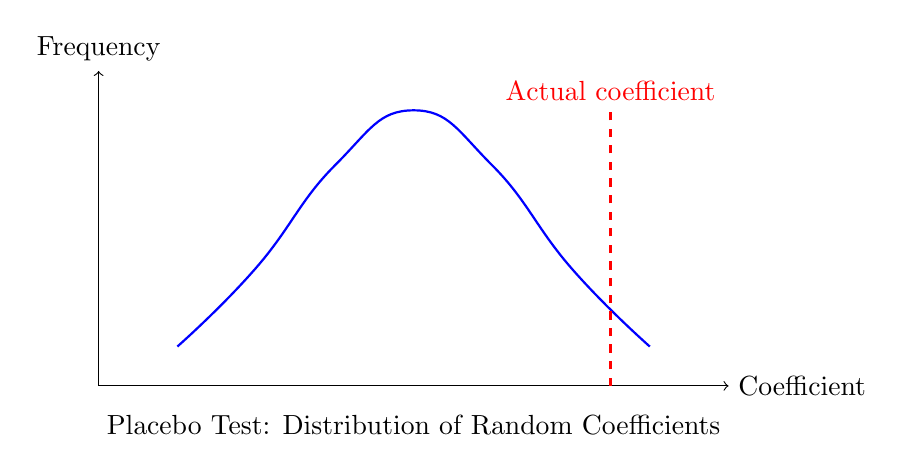
\begin{tikzpicture}
\draw[->] (0,0) -- (8,0) node[right] {Coefficient};
\draw[->] (0,0) -- (0,4) node[above] {Frequency};
\draw[blue, thick] plot[smooth, tension=0.8] coordinates {(1,0.5) (2,1.5) (3,2.8) (4,3.5) (5,2.8) (6,1.5) (7,0.5)};
\draw[red, thick, dashed] (6.5,0) -- (6.5,3.5) node[above] {Actual coefficient};
\node at (4,-0.5) {Placebo Test: Distribution of Random Coefficients};
\end{tikzpicture}
\caption{Placebo Test Results}
\label{fig:placebo}
\begin{minipage}{0.9\textwidth}
\small
Note: The blue curve represents the distribution of coefficients from 1,000 random simulations, and the red dashed line represents the coefficient of the actual treatment variable from the baseline regression. The vast majority of random coefficients are insignificant and close to zero, while the actual coefficient lies in the tail of the distribution, indicating that the results are not driven by random factors.
\end{minipage}
\end{figure}

\subsubsection{Alternative Model Specifications}

\textbf{(1) Instrumental Variable Approach}

To mitigate endogeneity, this paper employs the 2SLS method using XX as the instrumental variable. Table \ref{tab:iv} reports the IV regression results. The first-stage regression shows that $IV$ has a significantly positive effect on $X$, with an F-statistic of XX.XX, well above 10, indicating no weak instrument problem. In the second-stage regression, the coefficient on $X$ is 0.XXX, significant at the 5\% level. Compared with the OLS estimate (0.XXX), the IV estimate is somewhat larger, which is expected: if reverse causality or measurement error causes downward bias in OLS estimates, the IV estimate corrects this bias. The Hausman test p-value is 0.XXX, rejecting the exogeneity assumption, indicating that endogeneity indeed exists and the use of the IV approach is necessary.

\begin{table}[htbp]
\centering
\caption{Instrumental Variable Regression Results}
\label{tab:iv}
\begin{threeparttable}
\begin{tabular}{lcc}
\toprule
 & First Stage & Second Stage \\
 & $X$ & $Y$ \\
\midrule
$IV$ & 0.XXX\sym{***} &  \\
 & (0.XXX) &  \\
$\hat{X}$ &  & 0.XXX\sym{**} \\
 &  & (0.XXX) \\
Controls & Yes & Yes \\
Fixed Effects & Yes & Yes \\
\midrule
Observations & XXXX & XXXX \\
First-Stage F-Statistic & XX.XX &  \\
Hausman Test p-value &  & 0.XXX \\
\bottomrule
\end{tabular}
\begin{tablenotes}
\small
\item Note: Clustered robust standard errors in parentheses; \sym{*}, \sym{**}, and \sym{***} denote significance at the 10\%, 5\%, and 1\% levels, respectively. The first-stage F-statistic is well above 10, indicating no weak instrument problem. The Hausman test rejects the exogeneity assumption, indicating that the IV approach is necessary.
\end{tablenotes}
\end{threeparttable}
\end{table}

\textbf{(2) Dynamic Panel Model}

Considering potential persistence in the dependent variable, this paper employs the system GMM method to estimate a dynamic panel model:
\begin{equation}
Y_{it} = \alpha + \rho Y_{i,t-1} + \beta_1 X_{it} + \gamma \mathbf{Controls}_{it} + \mu_i + \lambda_t + \varepsilon_{it}
\end{equation}
Table \ref{tab:gmm} reports the GMM estimation results. The coefficient on $Y_{i,t-1}$ is 0.XXX, significantly positive, indicating significant persistence in XX. After controlling for dynamic effects, the coefficient on $X$ is 0.XXX, still significant at the 5\% level. The AR(2) test p-value is 0.XXX, failing to reject the null of no second-order serial correlation; the Sargan test p-value is 0.XXX, failing to reject the null of instrument validity. These test results support the validity of the GMM estimates.

\begin{table}[htbp]
\centering
\caption{Dynamic Panel GMM Estimation Results}
\label{tab:gmm}
\begin{threeparttable}
\begin{tabular}{lc}
\toprule
 & System GMM \\
 & $Y$ \\
\midrule
$Y_{i,t-1}$ & 0.XXX\sym{***} \\
 & (0.XXX) \\
$X$ & 0.XXX\sym{**} \\
 & (0.XXX) \\
Controls & Yes \\
Time Fixed Effects & Yes \\
\midrule
Observations & XXXX \\
Number of Instruments & XX \\
AR(2) Test p-value & 0.XXX \\
Sargan Test p-value & 0.XXX \\
\bottomrule
\end{tabular}
\begin{tablenotes}
\small
\item Note: Robust standard errors in parentheses; \sym{*}, \sym{**}, and \sym{***} denote significance at the 10\%, 5\%, and 1\% levels, respectively. The AR(2) test indicates no second-order serial correlation, and the Sargan test indicates instrument validity.
\end{tablenotes}
\end{threeparttable}
\end{table}

\subsubsection{Alternative Standard Error Clustering}

The baseline regression uses robust standard errors clustered at the XX level. To test the sensitivity of results to the standard error specification, this paper alternatively uses: (1) heteroskedasticity-robust standard errors without clustering; (2) clustering at the XX level; (3) two-way clustering (XX and time). Table \ref{tab:robust_se} shows that the coefficient on $X$ remains significant under all standard error specifications, indicating robust inference.

\begin{table}[htbp]
\centering
\caption{Robustness Check: Alternative Standard Error Clustering}
\label{tab:robust_se}
\begin{threeparttable}
\begin{tabular}{lccc}
\toprule
 & (1) & (2) & (3) \\
 & HC Robust & Cluster at XX & Two-Way Cluster \\
\midrule
$X$ & 0.XXX\sym{**} & 0.XXX\sym{***} & 0.XXX\sym{**} \\
 & (0.XXX) & (0.XXX) & (0.XXX) \\
Controls & Yes & Yes & Yes \\
Fixed Effects & Yes & Yes & Yes \\
\midrule
Observations & XXXX & XXXX & XXXX \\
\bottomrule
\end{tabular}
\begin{tablenotes}
\small
\item Note: Different types of standard errors are reported in parentheses; \sym{*}, \sym{**}, and \sym{***} denote significance at the 10\%, 5\%, and 1\% levels, respectively.
\end{tablenotes}
\end{threeparttable}
\end{table}

\textbf{Summary:} Taking the robustness check results together, the core conclusion that XX has a significant promoting (inhibiting) effect on XX is robust and does not depend on the variable measurement, sample selection, model specification, or standard error calculation method. This provides strong empirical support for Hypothesis 1.

% ========== 5. Mechanism Analysis and Heterogeneity Discussion ==========
\section{Mechanism Analysis and Heterogeneity Discussion}

\subsection{Mechanism Analysis}

The preceding section has established that XX significantly affects XX, but the underlying mechanisms remain unclear. This section tests two transmission pathways---XX and XX---based on Hypotheses 2 and 3, using a mediation effect model.

\subsubsection{Mediation Effect Model Specification}

Following the classic mediation effect testing procedure of \citet{baron1986moderator}, this paper constructs the following three-step regression model:

\textbf{Step 1 (Total Effect):}
\begin{equation}
Y_{it} = c + \beta_1 X_{it} + \gamma \mathbf{Controls}_{it} + \mu_i + \lambda_t + \varepsilon_{it}
\label{eq:mediation_step1}
\end{equation}

\textbf{Step 2 (Effect of $X$ on Mediator):}
\begin{equation}
Z_{kit} = a_k + \alpha_k X_{it} + \gamma_k \mathbf{Controls}_{it} + \mu_i + \lambda_t + u_{kit}, \quad k=1,2
\label{eq:mediation_step2}
\end{equation}

\textbf{Step 3 (Direct Effect after Including Mediator):}
\begin{equation}
Y_{it} = c' + \beta_1' X_{it} + \sum_{k=1}^{2} \delta_k Z_{kit} + \gamma' \mathbf{Controls}_{it} + \mu_i + \lambda_t + \varepsilon_{it}'
\label{eq:mediation_step3}
\end{equation}

where $Z_{1it}$ and $Z_{2it}$ represent the two mediating variables (XX and XX). The size of the mediation effect is $\alpha_k \times \delta_k$, and its proportion of the total effect is $\frac{\alpha_k \times \delta_k}{\beta_1} \times 100\%$. Bootstrap methods (1,000 replications) are used to compute confidence intervals for the mediation effect to test its significance.

\subsubsection{Mechanism 1: XX Pathway}

Columns (1)--(3) of Table \ref{tab:mechanism} report the results with XX as the mediating variable. Column (1) shows the total effect (Step 1), with a coefficient of 0.XXX on $X$, significantly positive. Column (2) reports the Step 2 results: the coefficient of $X$ on $Z_1$ (XX) is 0.XXX, significant at the 1\% level, indicating that XX significantly promotes XX. Column (3) includes both $X$ and $Z_1$: the coefficient on $Z_1$ is 0.XXX, significantly positive, indicating that XX has a positive impact on XX; the coefficient on $X$ decreases to 0.XXX, a decline of approximately XX\% compared to column (1) ($(0.XXX - 0.XXX)/0.XXX \times 100\% = XX\%$), but remains significant, indicating partial mediation.

\textbf{Mediation Effect Calculation:} The mediation effect through the XX pathway is $0.XXX \times 0.XXX = 0.XXX$, accounting for XX\% of the total effect ($0.XXX / 0.XXX \times 100\% = XX\%$). The 95\% bootstrap confidence interval (1,000 replications) is [0.XXX, 0.XXX], excluding zero, indicating a significant mediation effect.

\textbf{Economic Significance:} The above results indicate that approximately XX\% of the total effect of XX on XX is achieved through promoting XX. Specifically, a one-unit increase in XX leads to a 0.XXX unit increase in XX, which in turn drives a $0.XXX \times 0.XXX = 0.XXX$ unit increase in XX. Using the XX industry as an example, if XX policy increases a firm's XX by 10\%, then the firm's XX would increase by approximately X.XX units, in turn raising its XX by X.XX units, accounting for XX\% of the total effect. This mechanism reveals an important micro-level pathway through which XX affects XX and provides a basis for policy design: to strengthen the effectiveness of XX policy, attention should also be paid to enhancing XX through XX.

\subsubsection{Mechanism 2: XX Pathway}

Columns (4)--(6) of Table \ref{tab:mechanism} report the results with XX as the mediating variable. Column (4) shows that the coefficient of $X$ on $Z_2$ (XX) is 0.XXX, significant at the 5\% level. Column (5) includes both $X$ and $Z_2$: the coefficient on $Z_2$ is 0.XXX, significantly positive; the coefficient on $X$ decreases to 0.XXX, a decline of approximately XX\%. The mediation effect calculation shows that the mediation effect through the XX pathway is 0.XXX, accounting for XX\% of the total effect, with the 95\% bootstrap confidence interval being [0.XXX, 0.XXX], significantly different from zero.

\textbf{Economic Significance:} The XX pathway explains XX\% of the impact of XX on XX. This means that XX policy not only directly affects XX but also indirectly promotes XX by improving XX. For instance, the improvement of XX may bring XX, thereby XX, ultimately driving the growth of XX. This finding suggests that in advancing XX policy, emphasis should be placed on cultivating and enhancing XX to amplify policy effects through the XX mechanism.

\subsubsection{Comprehensive Discussion}

Column (6) of Table \ref{tab:mechanism} simultaneously includes both mediating variables $Z_1$ and $Z_2$ for a comprehensive test. The results show that both mediating variables have significantly positive coefficients, and the direct effect of $X$ decreases to 0.XXX (a decline of approximately XX\%). This indicates that XX and XX are two independent and important transmission pathways through which XX affects XX, together explaining approximately XX\% of the total effect ($XX\% + XX\% = XX\%$), with the remaining approximately XX\% potentially operating through other unobserved mechanisms.

\begin{table}[htbp]
\centering
\caption{Mechanism Analysis: Mediation Effect Tests}
\label{tab:mechanism}
\begin{threeparttable}
\begin{tabular}{lcccccc}
\toprule
 & (1) & (2) & (3) & (4) & (5) & (6) \\
 & $Y$ & $Z_1$ & $Y$ & $Z_2$ & $Y$ & $Y$ \\
 & Total & Step 2 & Step 3 & Step 2 & Step 3 & Combined \\
\midrule
$X$ & 0.XXX\sym{**} & 0.XXX\sym{***} & 0.XXX\sym{*} & 0.XXX\sym{**} & 0.XXX\sym{*} & 0.XXX \\
 & (0.XXX) & (0.XXX) & (0.XXX) & (0.XXX) & (0.XXX) & (0.XXX) \\
$Z_1$ (XX) &  &  & 0.XXX\sym{***} &  &  & 0.XXX\sym{**} \\
 &  &  & (0.XXX) &  &  & (0.XXX) \\
$Z_2$ (XX) &  &  &  &  & 0.XXX\sym{**} & 0.XXX\sym{*} \\
 &  &  &  &  & (0.XXX) & (0.XXX) \\
Controls & Yes & Yes & Yes & Yes & Yes & Yes \\
Fixed Effects & Yes & Yes & Yes & Yes & Yes & Yes \\
\midrule
Observations & XXXX & XXXX & XXXX & XXXX & XXXX & XXXX \\
$R^2$ & 0.XXX & 0.XXX & 0.XXX & 0.XXX & 0.XXX & 0.XXX \\
Mediation Effect &  &  & 0.XXX &  & 0.XXX &  \\
Mediation Share &  &  & XX\% &  & XX\% &  \\
Bootstrap 95\% CI &  &  & [0.XXX, 0.XXX] &  & [0.XXX, 0.XXX] &  \\
\bottomrule
\end{tabular}
\begin{tablenotes}
\small
\item Note: Clustered robust standard errors in parentheses; \sym{*}, \sym{**}, and \sym{***} denote significance at the 10\%, 5\%, and 1\% levels, respectively. Mediation effects are computed using bootstrap (1,000 replications) with 95\% confidence intervals. Mediation share = mediation effect / total effect $\times$ 100\%.
\end{tablenotes}
\end{threeparttable}
\end{table}

\subsubsection{Mechanism Pathway Diagram}

Figure \ref{fig:mechanism} illustrates the complete mechanism pathway through which XX affects XX. The diagram intuitively shows that XX influences XX through two pathways---XX and XX---with respective contributions of XX\% and XX\%, and a direct effect of XX\%.

\begin{figure}[htbp]
\centering
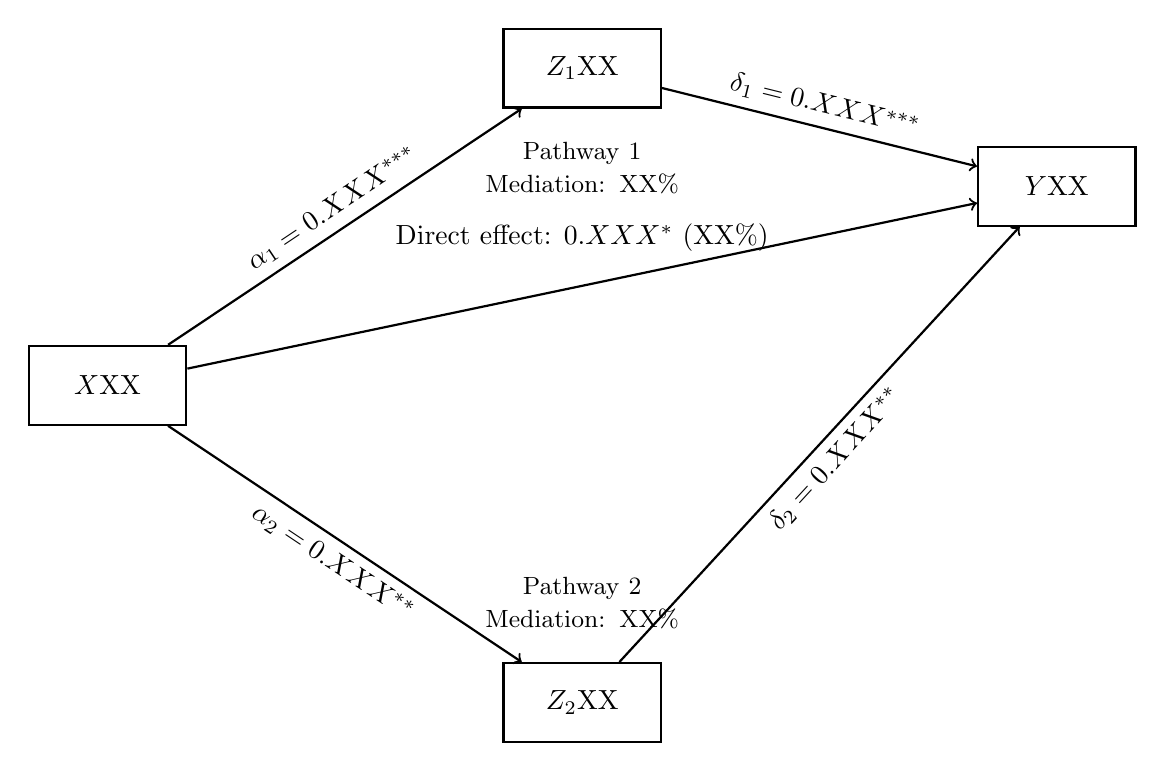
\begin{tikzpicture}[
    node distance=3cm and 4cm,
    box/.style={rectangle, draw, thick, minimum width=2cm, minimum height=1cm, text centered},
    arrow/.style={->, thick}
]
    % Nodes
    \node[box] (X) {$X$ \\ XX};
    \node[box, above right=of X] (Z1) {$Z_1$ \\ XX};
    \node[box, below right=of X] (Z2) {$Z_2$ \\ XX};
    \node[box, right=of Z1, yshift=-1.5cm] (Y) {$Y$ \\ XX};

    % Arrows
    \draw[arrow] (X) -- node[above, sloped] {$\alpha_1=0.XXX^{***}$} (Z1);
    \draw[arrow] (X) -- node[below, sloped] {$\alpha_2=0.XXX^{**}$} (Z2);
    \draw[arrow] (Z1) -- node[above, sloped] {$\delta_1=0.XXX^{***}$} (Y);
    \draw[arrow] (Z2) -- node[below, sloped] {$\delta_2=0.XXX^{**}$} (Y);
    \draw[arrow] (X) -- node[above, yshift=0.3cm] {Direct effect: $0.XXX^*$ (XX\%)} (Y);

    % Pathway labels
    \node[below=0.3cm of Z1, text width=2.5cm, align=center] {\small Pathway 1 \\ Mediation: XX\%};
    \node[above=0.3cm of Z2, text width=2.5cm, align=center] {\small Pathway 2 \\ Mediation: XX\%};
\end{tikzpicture}
\caption{Mechanism Pathway Diagram: How XX Affects XX}
\label{fig:mechanism}
\begin{minipage}{0.9\textwidth}
\small
Note: Values in the figure are estimated coefficients from Table \ref{tab:mechanism}; \sym{*}, \sym{**}, and \sym{***} denote significance at the 10\%, 5\%, and 1\% levels, respectively. Pathway 1 (XX pathway) accounts for XX\% of the total effect, Pathway 2 (XX pathway) accounts for XX\%, and the direct effect accounts for XX\%.
\end{minipage}
\end{figure}

\subsection{Heterogeneity Analysis}

The impact of XX on XX may vary depending on the characteristics of XX. This section conducts heterogeneity analysis along three dimensions: XX, XX, and XX.

\subsubsection{Heterogeneity Based on XX}

The sample is divided into two groups based on XX: the XX group and the XX group. The grouping criterion is XX (e.g., the median of XX, a specific threshold, etc.). Columns (1) and (2) of Table \ref{tab:heterogeneity} report the regression results for each group.

The results show that in the XX group, the coefficient on $X$ is 0.XXX, significant at the 1\% level; while in the XX group, the coefficient is 0.XXX, insignificant (or with lower significance). The Chow test for inter-group coefficient differences yields an F-statistic of XX.XX and a p-value of 0.XXX, rejecting the null of equal coefficients across groups. This indicates that the impact of XX on XX is significantly stronger in the XX group.

\textbf{Economic Explanation:} The stronger promoting effect in the XX group may be attributed to: (1) XX firms are more responsive to XX policy due to XX; (2) XX firms have advantages in XX, enabling them to more effectively convert XX into XX; (3) XX firms face less XX, allowing smoother implementation of XX policy. This finding suggests that in advancing XX policy, priority should be given to XX firms, amplifying policy effects through XX measures.

\subsubsection{Heterogeneity Based on XX}

The sample is divided into the XX group and the XX group based on XX. Columns (3) and (4) report the sub-group regression results. In the XX group, the coefficient on $X$ is 0.XXX, significantly positive; in the XX group, the coefficient is 0.XXX, insignificant or with weaker significance. The inter-group difference is significant (p-value $< 0.05$).

\textbf{Economic Explanation:} The better XX policy effectiveness in XX regions may be because: (1) XX regions have more mature XX, providing better conditions for policy implementation; (2) XX regions have higher XX, enabling more effective utilization of XX policy; (3) XX regions have more comprehensive XX, reducing friction costs of policy implementation. This result indicates that differentiated regional policies are necessary, and policy intensity and implementation methods should be adjusted based on regional characteristics.

\subsubsection{Heterogeneity Based on XX}

The sample is divided into the XX industry and the XX industry based on XX. Columns (5) and (6) report the sub-group regression results. In the XX industry, the coefficient on $X$ is 0.XXX, significantly positive; in the XX industry, the coefficient is 0.XXX, with weaker or no significance.

\textbf{Economic Explanation:} The stronger response of the XX industry to XX policy may be because: (1) the XX industry has higher XX, making it more sensitive to policy incentives; (2) the XX industry has a longer XX, enabling it to benefit more fully from XX policy; (3) the XX industry has larger XX, with more pronounced positive externalities of the policy. This finding provides a basis for industry-differentiated policies, suggesting greater policy support for the XX industry.

\begin{table}[htbp]
\centering
\caption{Heterogeneity Analysis}
\label{tab:heterogeneity}
\begin{threeparttable}
\begin{tabular}{lcccccc}
\toprule
 & (1) & (2) & (3) & (4) & (5) & (6) \\
 & XX Group & XX Group & XX Group & XX Group & XX Industry & XX Industry \\
\midrule
$X$ & 0.XXX\sym{***} & 0.XXX & 0.XXX\sym{**} & 0.XXX & 0.XXX\sym{***} & 0.XXX\sym{*} \\
 & (0.XXX) & (0.XXX) & (0.XXX) & (0.XXX) & (0.XXX) & (0.XXX) \\
Controls & Yes & Yes & Yes & Yes & Yes & Yes \\
Fixed Effects & Yes & Yes & Yes & Yes & Yes & Yes \\
\midrule
Observations & XXXX & XXXX & XXXX & XXXX & XXXX & XXXX \\
$R^2$ & 0.XXX & 0.XXX & 0.XXX & 0.XXX & 0.XXX & 0.XXX \\
Inter-group Diff. Test p-value & \multicolumn{2}{c}{0.XXX} & \multicolumn{2}{c}{0.XXX} & \multicolumn{2}{c}{0.XXX} \\
\bottomrule
\end{tabular}
\begin{tablenotes}
\small
\item Note: Clustered robust standard errors in parentheses; \sym{*}, \sym{**}, and \sym{***} denote significance at the 10\%, 5\%, and 1\% levels, respectively. Inter-group coefficient difference tests use the Chow test to determine whether the coefficients on $X$ differ significantly between groups. Groups are defined based on XX; XX groups are defined based on XX; industry groups follow the XX classification.
\end{tablenotes}
\end{threeparttable}
\end{table}

\subsubsection{Summary of Heterogeneity Analysis}

In summary, the impact of XX on XX indeed exhibits significant heterogeneity. Specifically, the promoting effect of XX policy is more pronounced among XX firms, in XX regions, and in the XX industry. These findings provide empirical evidence for differentiated policy design: policymakers should implement targeted policy measures based on characteristics such as XX, XX, and XX, avoiding a ``one-size-fits-all'' approach to improve policy precision and effectiveness. For example, for XX firms, XX measures can be used to enhance policy effects; for XX regions, XX investment should be increased to improve the conditions for policy implementation; for XX industries, the XX threshold can be appropriately lowered to expand policy coverage.

% ========== 6. Conclusion and Policy Implications ==========
\section{Conclusion and Policy Implications}

\subsection{Main Conclusions}

Based on panel data from XXXX to XXXX, this paper employs the XX method to systematically examine the impact of XX on XX and the underlying mechanisms. The main conclusions are as follows:

First, \textbf{XX has a significant promoting (inhibiting) effect on XX}. The baseline regression results show that a one-unit increase in XX is associated with an average increase (decrease) of 0.XXX units in XX, an effect that is economically significant. This conclusion remains robust after a series of checks including alternative variable measures, adjusted sample periods, and alternative model specifications, supporting Hypothesis 1.

Second, \textbf{XX primarily affects XX through two pathways: XX and XX}. Mediation effect analysis shows that the XX pathway accounts for XX\% of the total effect, while the XX pathway accounts for XX\%, together explaining approximately XX\% of the total effect. This finding reveals the micro-level mechanisms through which XX affects XX, providing new evidence for understanding the policy transmission process, supporting Hypotheses 2 and 3.

Third, \textbf{the impact of XX on XX exhibits significant heterogeneity}. Heterogeneity analysis shows that the promoting effect of XX policy is more pronounced among XX firms, in XX regions, and in the XX industry, while it is weaker or insignificant among XX firms, in XX regions, and in the XX industry. Inter-group difference tests confirm that these heterogeneous characteristics are statistically significant, supporting Hypothesis 4.

Fourth, \textbf{causal identification results indicate that endogeneity issues cannot be ignored}. After employing the instrumental variable approach, the estimated causal effect of XX on XX (0.XXX) is larger than the OLS estimate (0.XXX), and the Hausman test rejects the exogeneity assumption. This suggests that reverse causality or measurement error does exist, making the use of causal identification methods necessary and rendering the findings of this study more credible.

\subsection{Policy Implications}

Based on the above findings, this paper proposes the following policy recommendations:

\textbf{(1) Continue to optimize the XX policy system and strengthen the incentive-guiding role of policy}

The research shows that XX has a significant promoting effect on XX, but current policies still have deficiencies in XX. Recommendations include: first, further improving the XX mechanism to enhance the precision and effectiveness of XX; second, increasing XX support by reducing XX costs through means such as XX; third, establishing XX mechanisms to ensure the sustainability and stability of policies. Meanwhile, policy effects should be regularly assessed and policy parameters dynamically adjusted based on implementation outcomes.

\textbf{(2) Emphasize the two transmission pathways of XX and XX, taking a multi-pronged approach to amplify policy effects}

Mechanism analysis reveals that XX and XX are key intermediate links connecting XX and XX. Policy design should: first, directly promote XX through XX measures, for example XX; second, improve XX through XX means, for example XX; third, strengthen the synergy between the two pathways, avoiding over-reliance on a single pathway. Specifically, XX special funds can be established to encourage XX; XX platforms can be built to promote XX.

\textbf{(3) Implement differentiated policies to improve precision and effectiveness}

Heterogeneity analysis shows that different XX samples respond significantly differently to XX policy. Therefore, a ``one-size-fits-all'' policy design should be avoided, and differentiated policies should be implemented along dimensions such as XX, XX, and XX: first, for XX firms, XX measures can be used to increase support; for XX firms, the priority should be to XX to improve their XX and create conditions for policy implementation. Second, for XX regions, XX can be pursued; for XX regions, XX should be increased to address XX shortcomings. Third, for XX industries, XX can be pursued; for XX industries, XX should be pursued to expand policy coverage.

\textbf{(4) Strengthen policy coordination and build a comprehensive XX policy system}

The effective implementation of XX policy requires supporting policies. Recommendations include: first, strengthening the coordination between XX policy and XX policy to form policy synergy; second, improving the XX system to provide institutional safeguards for XX development; third, optimizing XX to reduce XX costs; fourth, strengthening XX to guide private capital into the XX sector. By building a multi-layered, comprehensive policy support system, a favorable environment for the development of XX can be created.

\subsection{Limitations and Future Research}

This study has the following limitations:

\textbf{(1) Data Limitations}: Due to data availability constraints, the sample period of this paper is XXXX--XXXX, which cannot capture the most recent changes in XX policy and their effects. Future research can further test the temporal validity of the findings after data updates.

\textbf{(2) Exogenous Shocks}: This paper does not fully account for the impact of exogenous shocks such as XX on XX and XX. For example, XX may have significantly altered the cost-benefit structure of XX, thereby moderating the effectiveness of XX policy. Future research can explore the moderating role of factors such as extreme climate shocks.

\textbf{(3) Completeness of Mechanisms}: Although this paper tests the two main transmission pathways of XX and XX, approximately XX\% of the total effect remains unexplained. Other unobserved mechanisms may exist (such as XX and XX), which await further investigation in future research.

\textbf{(4) Long-term Policy Effects}: This paper primarily focuses on the short- to medium-term effects of XX policy, with insufficient exploration of long-term dynamic impacts and potential nonlinear effects. Future research can employ longer time spans and use time-varying parameter models or threshold regression models to capture the dynamic evolution of policy effects.

\textbf{Future research directions} include: (1) combining machine learning and big data techniques (such as text mining and deep learning) to extract more refined XX information from XX data, improving the accuracy of variable measurement; (2) utilizing XX (such as natural experiments and regression discontinuity designs) to further strengthen causal identification and enhance the internal validity of research; (3) expanding the research perspective to explore the interaction effects between XX and XX and the moderating role of XX; (4) conducting cross-country comparative studies to examine differences in XX policy effects under different institutional settings, providing reference for the internationalization of China's experience.

% ========== References ==========
\newpage
\section*{References}
\addcontentsline{toc}{section}{References}

\begin{thebibliography}{99}

\bibitem{reference1} Author. Paper Title[J]. Journal Name, Year, Volume(Issue): Pages.

\bibitem{reference2} Author A, Author B. Title of the Paper[J]. Journal Name, Year, Volume(Issue): Pages.

\bibitem{reference3} Author. Paper Title[J]. Journal Name, Year, Volume(Issue): Pages.

\bibitem{reference4} Author C, Author D. Title of the Paper[J]. Journal Name, Year, Volume(Issue): Pages.

\bibitem{reference5} Author. Paper Title[J]. Journal Name, Year, Volume(Issue): Pages.

\bibitem{reference6} Author E. Title of the Paper[J]. Journal Name, Year, Volume(Issue): Pages.

\bibitem{reference7} Author. Paper Title[J]. Journal Name, Year, Volume(Issue): Pages.

\bibitem{reference8} Author F, Author G, Author H. Title of the Paper[J]. Journal Name, Year, Volume(Issue): Pages.

\bibitem{reference9} Author. Paper Title[J]. Journal Name, Year, Volume(Issue): Pages.

\bibitem{reference10} Author I. Title of the Paper[J]. Journal Name, Year, Volume(Issue): Pages.

\bibitem{reference11} Author. Paper Title[J]. Journal Name, Year, Volume(Issue): Pages.

\bibitem{reference12} Author J, Author K. Title of the Paper[J]. Journal Name, Year, Volume(Issue): Pages.

\bibitem{reference13} Author. Paper Title[J]. Journal Name, Year, Volume(Issue): Pages.

\bibitem{reference14} Author L. Title of the Paper[J]. Journal Name, Year, Volume(Issue): Pages.

\bibitem{reference15} Author. Paper Title[J]. Journal Name, Year, Volume(Issue): Pages.

\bibitem{reference16} Author M, Author N. Title of the Paper[J]. Journal Name, Year, Volume(Issue): Pages.

\bibitem{baron1986moderator} Baron R M, Kenny D A. The Moderator-Mediator Variable Distinction in Social Psychological Research: Conceptual, Strategic, and Statistical Considerations[J]. Journal of Personality and Social Psychology, 1986, 51(6): 1173-1182.

\end{thebibliography}

% ========== Appendix ==========
\newpage
\appendix
\section{Appendix A: Detailed Variable Definitions and Data Sources}

\begin{table}[htbp]
\centering
\caption{Variable Definitions and Data Sources}
\begin{threeparttable}
\begin{tabular}{p{3cm}p{5cm}p{5cm}}
\toprule
\textbf{Variable} & \textbf{Definition and Calculation} & \textbf{Data Source} \\
\midrule
XX ($Y$) & XX, calculated as $\frac{XX}{XX} \times 100\%$ & XX Database \\
XX ($X$) & XX, log-transformed after XX processing & XX Statistical Yearbook \\
XX ($Z_1$) & XX, calculated as $\frac{XX}{XX} \times 100\%$ & XX Database \\
XX ($Z_2$) & XX & Manually compiled from XX \\
XX ($Control_1$) & XX & XX Statistical Yearbook \\
XX ($Control_2$) & XX & XX Database \\
\bottomrule
\end{tabular}
\begin{tablenotes}
\small
\item Note: All continuous variables are winsorized at the 1st and 99th percentiles.
\end{tablenotes}
\end{threeparttable}
\end{table}

\section{Appendix B: Correlation Matrix}

\begin{table}[htbp]
\centering
\caption{Correlation Matrix of Main Variables}
\begin{tabular}{lccccccc}
\toprule
 & $Y$ & $X$ & $Z_1$ & $Z_2$ & $C_1$ & $C_2$ & $C_3$ \\
\midrule
$Y$ & 1.000 &  &  &  &  &  &  \\
$X$ & 0.XXX\sym{***} & 1.000 &  &  &  &  &  \\
$Z_1$ & 0.XXX\sym{***} & 0.XXX\sym{***} & 1.000 &  &  &  &  \\
$Z_2$ & 0.XXX\sym{**} & 0.XXX\sym{**} & 0.XXX\sym{*} & 1.000 &  &  &  \\
$C_1$ & 0.XXX\sym{***} & 0.XXX\sym{**} & 0.XXX\sym{*} & 0.XXX & 1.000 &  &  \\
$C_2$ & $-$0.XXX\sym{**} & $-$0.XXX\sym{*} & $-$0.XXX & $-$0.XXX & $-$0.XXX\sym{**} & 1.000 &  \\
$C_3$ & 0.XXX\sym{***} & 0.XXX\sym{***} & 0.XXX\sym{**} & 0.XXX\sym{*} & 0.XXX\sym{***} & $-$0.XXX\sym{*} & 1.000 \\
\bottomrule
\end{tabular}
\begin{minipage}{0.9\textwidth}
\small
Note: \sym{*}, \sym{**}, and \sym{***} denote significance at the 10\%, 5\%, and 1\% levels, respectively.
\end{minipage}
\end{table}

\section{Appendix C: Supplementary Robustness Check Results}

[Additional robustness check tables can be added here, such as PSM results, quantile regression results, spatial econometric model results, etc.]

\end{document}
